\section{Motivational Example}
\label{sec:example}
\PUNT{
\begin{figure*}
  \subfloat[]
  {
    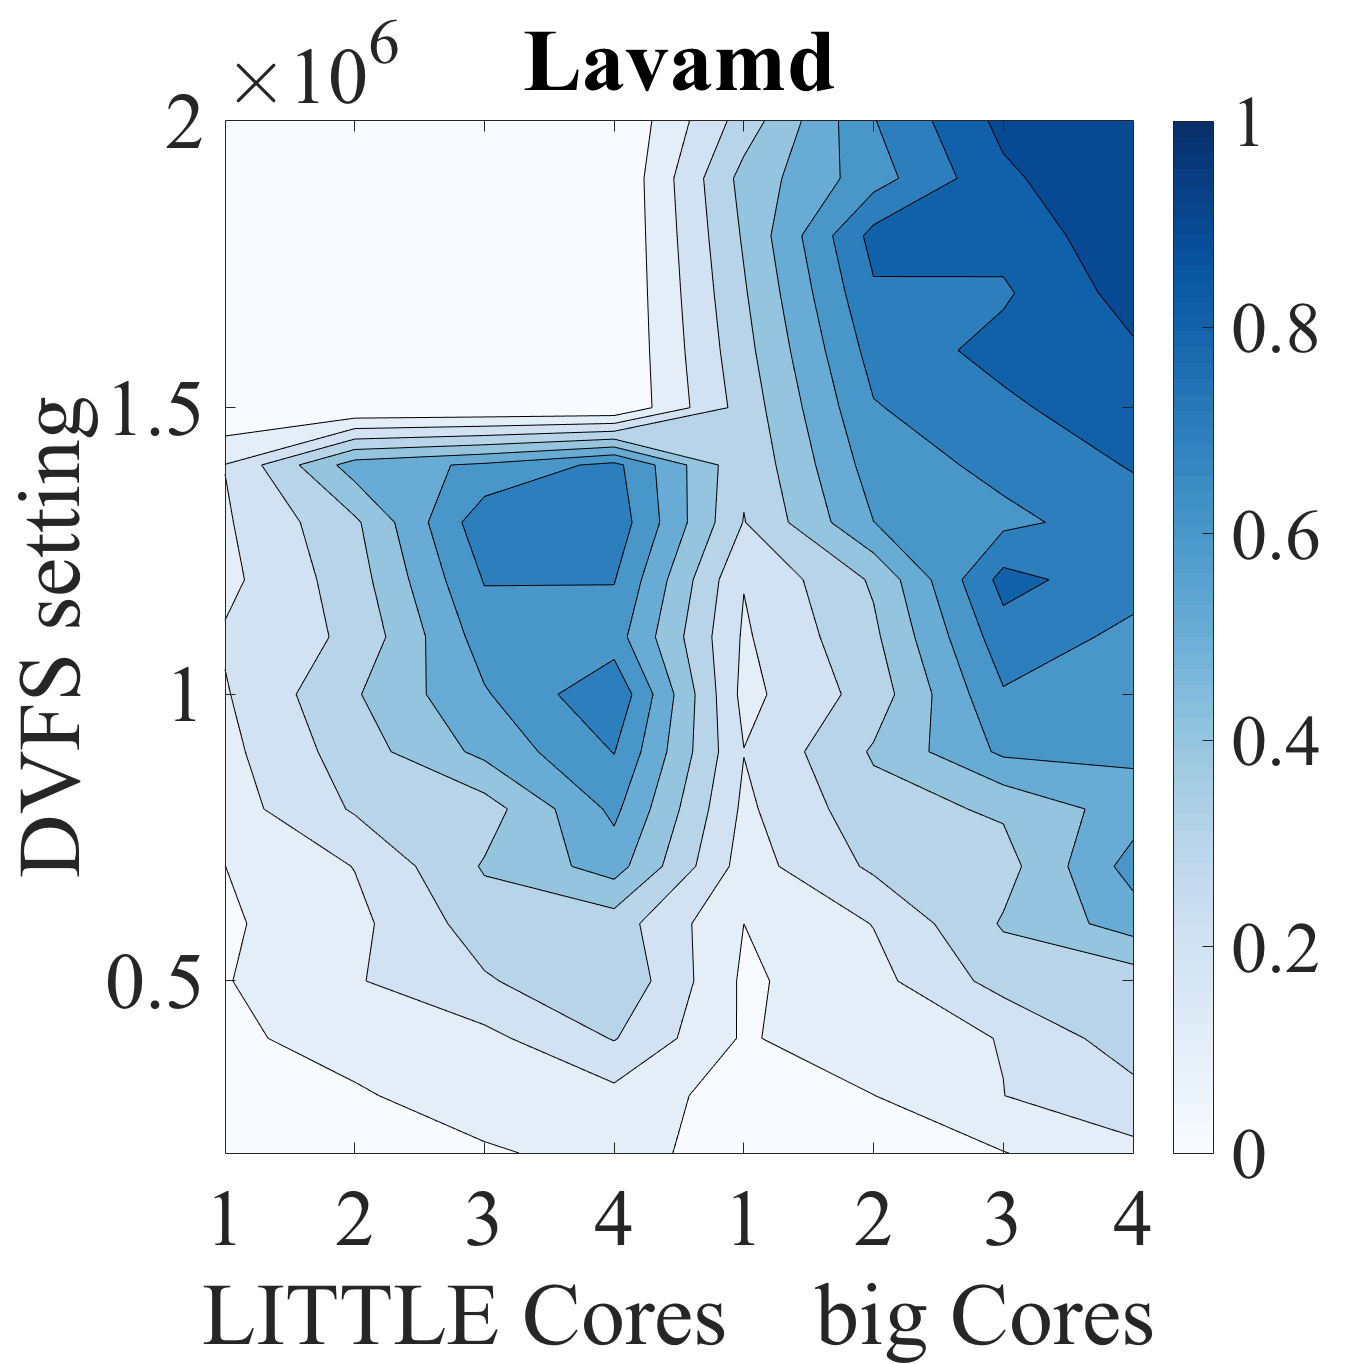
\includegraphics[width=.3\textwidth]{figures/lavamd.png}
    \label{fig:lavamd_contour}
  }
  \subfloat[]
  {
    \begin{tikzpicture}
\begin{centering}

\begin{groupplot}[
    group style={
        group name=plots,
        group size=1 by 1,
        xlabels at=edge bottom,
        xticklabels at=edge bottom,
        vertical sep=5pt
    },
height=4.1cm,
width=0.45\columnwidth,
xmajorgrids,
ymajorgrids,
grid style={dashed},
xmax=20,
yticklabel pos=left,
enlargelimits=false,
tick align = outside,
tick style={white},
xticklabel shift={-5pt},
yticklabel shift={-5pt},
ylabel shift={-2pt},
ylabel style={align=center},
unbounded coords=jump,
]

\nextgroupplot[ylabel={\scriptsize Performance (Normalized)}, % Performance
xlabel={\footnotesize Iteration},
ytick={0.0,0.5,1.0,1.5,2.0},
yticklabels={,0.25,0.5,1.0,1.5},
legend entries={,{\scriptsize $\mathsf{Generic~Model}$},{\scriptsize $\mathsf{LAVAMD model}$}},
legend style={fill=none,draw=none,at={(0.5,1.4)},anchor=north,legend columns=1,line width=3pt},
]

\addplot[thick, dashed, black] coordinates {(10,0) (10,1.5)};
\addplot[thick, solid, color=poet] table[x index=0,y index=1,col sep=tab] {img/image_text/lavamd-example.txt};
\addplot[thick, solid, color=cal] table[x index=0,y index=2,col sep=tab] {img/image_text/lavamd-example.txt};
\end{groupplot}
\end{centering}
\end{tikzpicture}
    \label{fig:lavamd_timeline}
  }
  \caption{(a) Contour plot for normalized performance for \texttt{Lavamd} algorithm for different configurations(b) Time-line for running \texttt{Lavamd}. \emph{Control} is running in isolation without an HBM based \emph{learning} mechanism which leads to oscillations in the performance.}
  \label{fig:learning-models}
\end{figure*}

\begin{figure}
  \subfloat[]
  {
    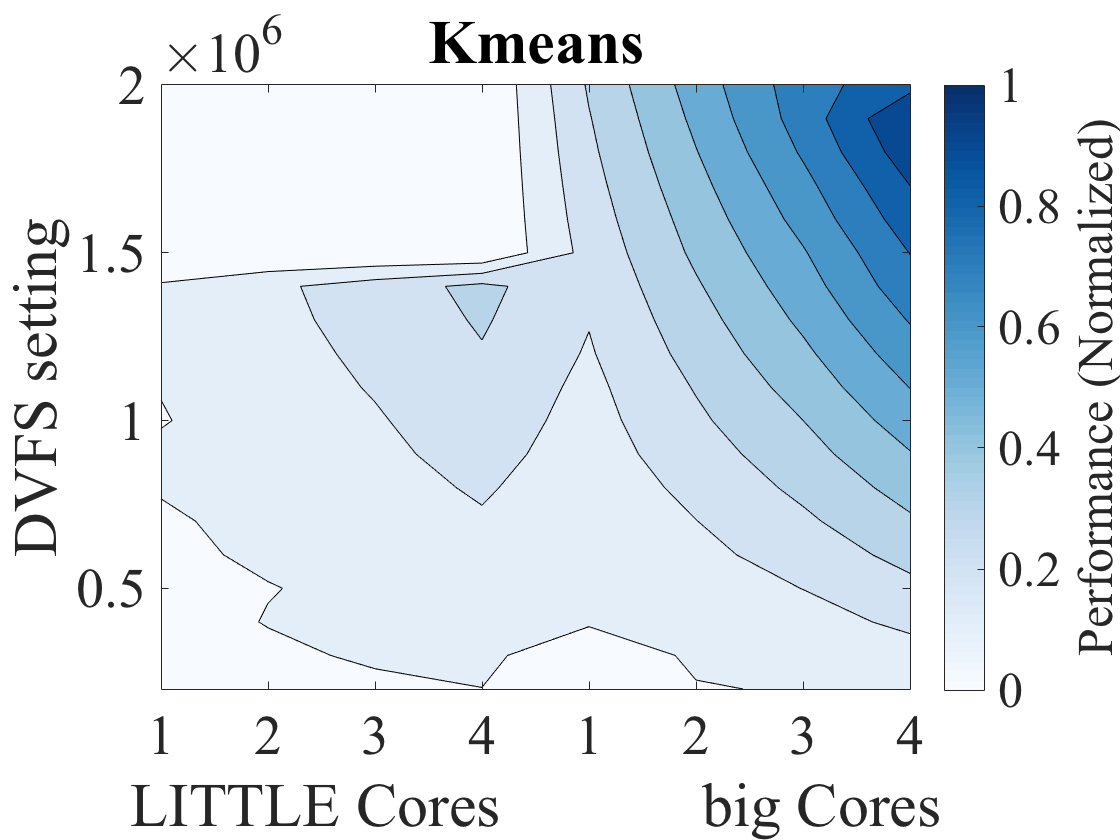
\includegraphics[width=.3\columnwidth]{figures/kmeans.png}
    \label{fig:kmeans_contour}
  }
  \subfloat[]
  {
    \begin{tikzpicture}
\begin{centering}

\definecolor{s1}{RGB}{228, 26, 28}
\definecolor{s2}{RGB}{55, 126, 184}
\definecolor{s3}{RGB}{77, 175, 74}
\definecolor{s4}{RGB}{152, 78, 163}
\definecolor{s5}{RGB}{255, 127, 0}

\begin{groupplot}[
    group style={
        group name=plots,
        group size=1 by 1,
        xlabels at=edge bottom,
        xticklabels at=edge bottom,
        vertical sep=5pt
    },
height=4cm,
width=1.3\columnwidth,
xmajorgrids,
ymajorgrids,
grid style={dashed},
xmin=0,
xmax=20,
yticklabel pos=left,
enlargelimits=false,
tick align = outside,
tick style={white},
xticklabel shift={-5pt},
yticklabel shift={-5pt},
ylabel shift={-2pt},
ylabel style={align=center},
unbounded coords=jump,
]

\nextgroupplot[ylabel={\footnotesize Performance \\ (Normalized)}, % Performance
%xtick={0,500,1000,1500,2000,2500,3000,3500,4000,4500},
ytick={0.0,0.5,1.0,1.5,2.0},
yticklabels={,0.5,1.0,1.5,2.0},
%xtick={0,30,60,120,160,200,240,280,320,480},
%xticklabels={,0,30,60,120,160,200,240,280,320,480},
%yticklabel style={font=\footnotesize},
xlabel={\footnotesize time (in sec)},
ymin=0,
ymax=1.5,
legend entries={,{$\mathsf{Learning}$},{$\mathsf{Control}$}},
legend style={draw=none,at={(0.5,1.3)},anchor=north,legend columns=4,
line width=5pt},
]

\addplot[thick, dashed, black] coordinates {(10,0) (10,1.5)};
\addplot[thick, solid, color=s4] table[x index=0,y index=1,col sep=tab] {img/image_text/kmeans-example.txt};
\addplot[thick, solid, color=s5] table[x index=0,y index=2,col sep=tab] {img/image_text/kmeans-example.txt};
%\addplot[thick, dashed, black] coordinates {(130,0) (130, 2)};
\end{groupplot}
\end{centering}

\end{tikzpicture}

    \label{fig:kmeans_timeline}    
  }
  \caption{(a) Contour plot for normalized performance for \texttt{Kmeans} algorithm for different configurations(b) Time-line for running \texttt{Kmeans} alone until 10 seconds, when another application. \emph{Learning} is running in isolation without an LCS based \emph{control} mechanism which leads to a performance drop which does not recover by itself.}
  \label{fig:learning-models}
\end{figure}
}
\begin{figure*}
  \subfloat[]
  {
    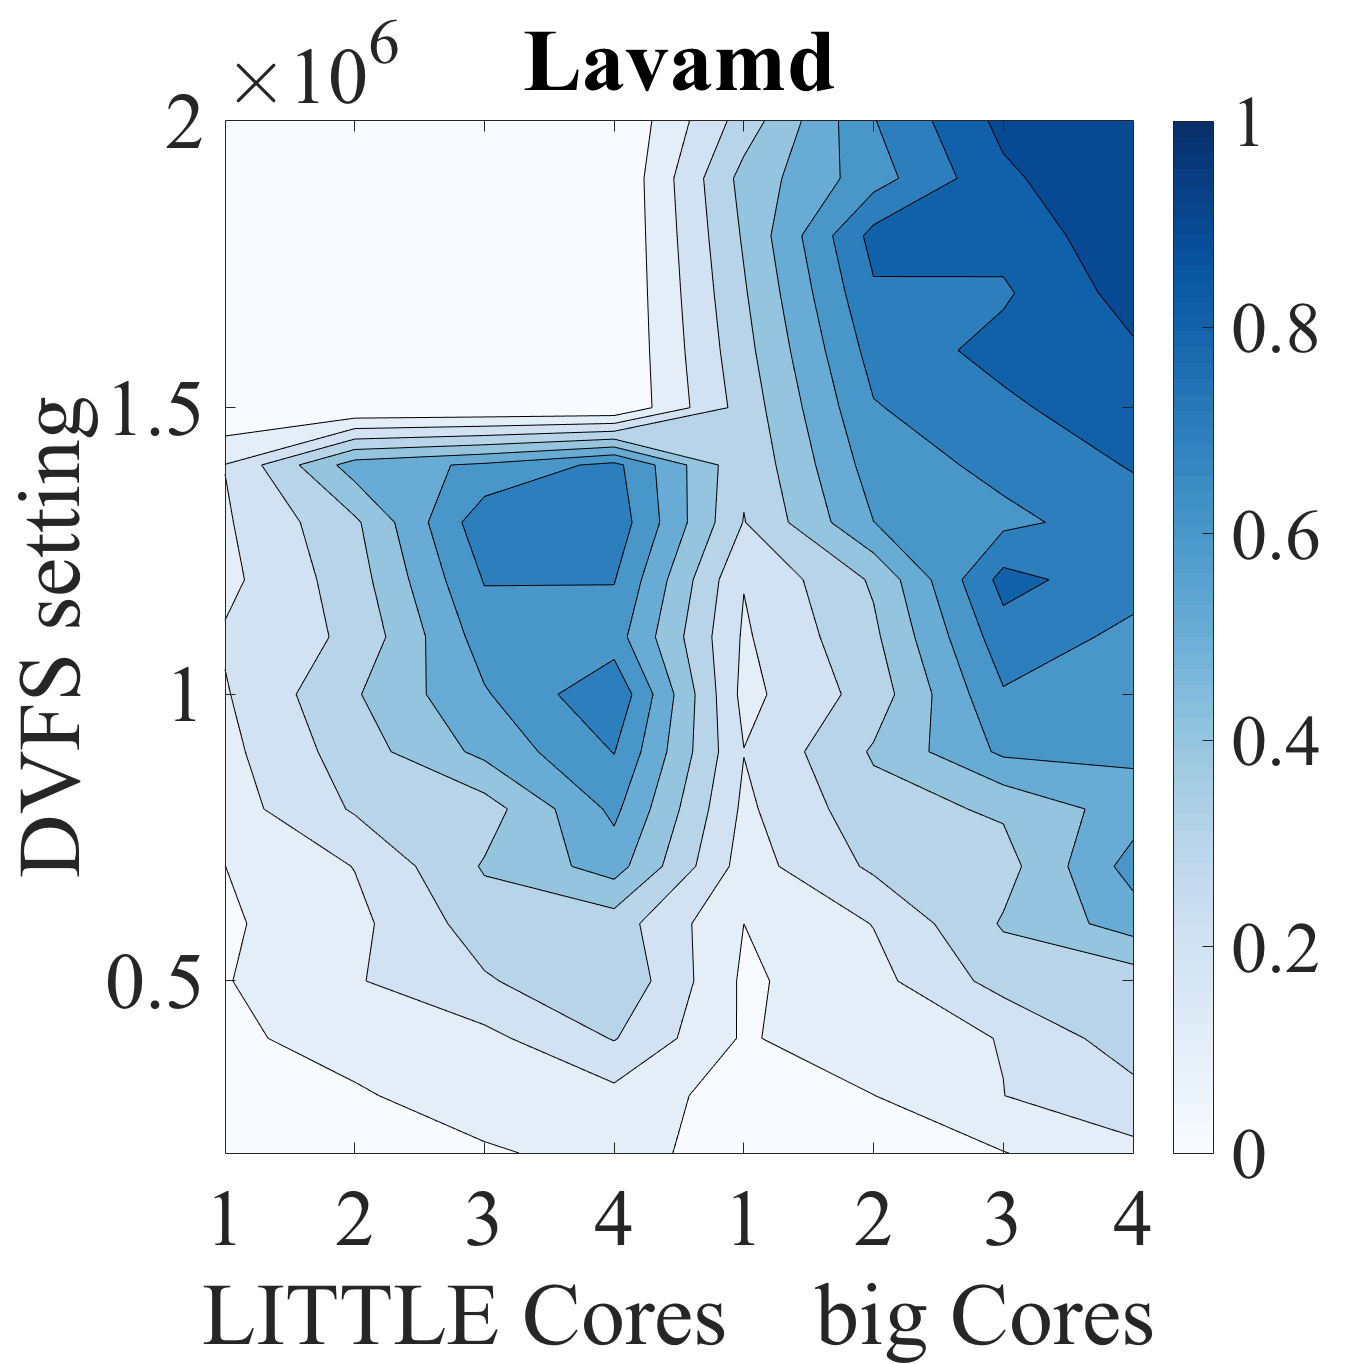
\includegraphics[width=.25\textwidth]{figures/lavamd.png}
    \label{fig:lavamd_contour}
  }
  \subfloat[]
  {
    \begin{tikzpicture}
\begin{centering}

\begin{groupplot}[
    group style={
        group name=plots,
        group size=1 by 1,
        xlabels at=edge bottom,
        xticklabels at=edge bottom,
        vertical sep=5pt
    },
height=4.1cm,
width=0.45\columnwidth,
xmajorgrids,
ymajorgrids,
grid style={dashed},
xmax=20,
yticklabel pos=left,
enlargelimits=false,
tick align = outside,
tick style={white},
xticklabel shift={-5pt},
yticklabel shift={-5pt},
ylabel shift={-2pt},
ylabel style={align=center},
unbounded coords=jump,
]

\nextgroupplot[ylabel={\scriptsize Performance (Normalized)}, % Performance
xlabel={\footnotesize Iteration},
ytick={0.0,0.5,1.0,1.5,2.0},
yticklabels={,0.25,0.5,1.0,1.5},
legend entries={,{\scriptsize $\mathsf{Generic~Model}$},{\scriptsize $\mathsf{LAVAMD model}$}},
legend style={fill=none,draw=none,at={(0.5,1.4)},anchor=north,legend columns=1,line width=3pt},
]

\addplot[thick, dashed, black] coordinates {(10,0) (10,1.5)};
\addplot[thick, solid, color=poet] table[x index=0,y index=1,col sep=tab] {img/image_text/lavamd-example.txt};
\addplot[thick, solid, color=cal] table[x index=0,y index=2,col sep=tab] {img/image_text/lavamd-example.txt};
\end{groupplot}
\end{centering}
\end{tikzpicture}
    \label{fig:lavamd_timeline}
  }
  \subfloat[]
  {
    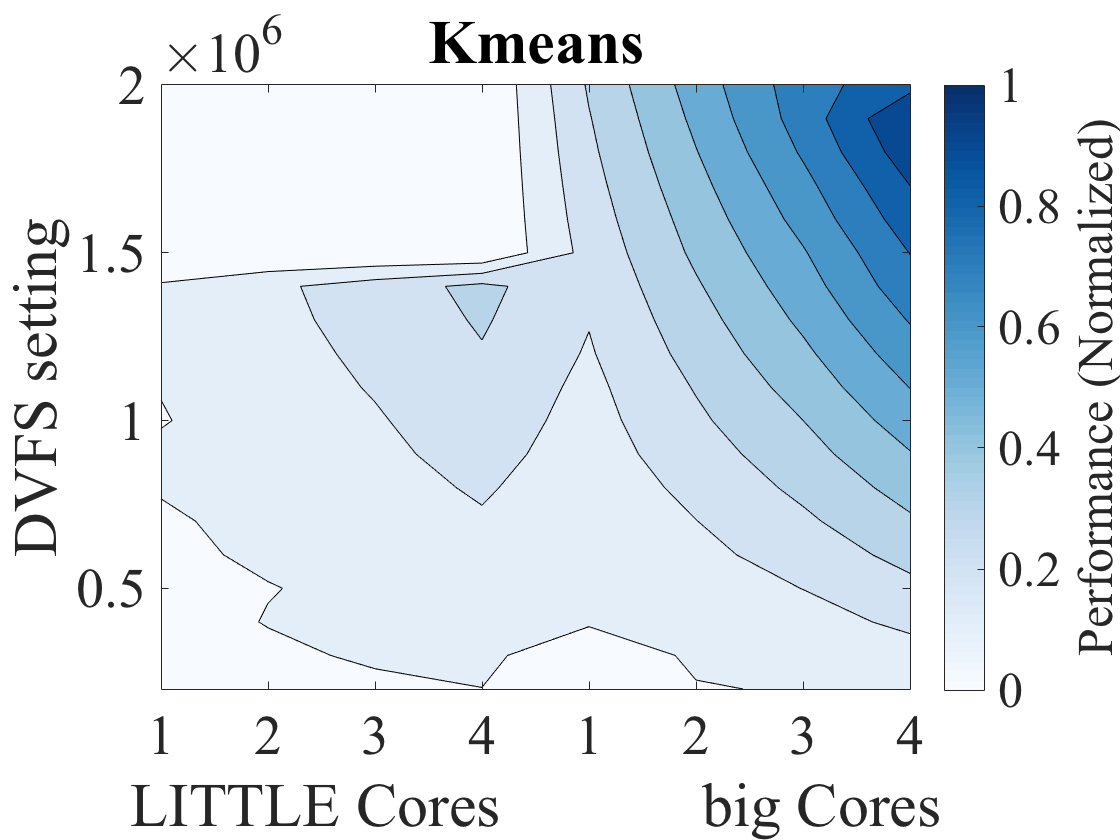
\includegraphics[width=.25\textwidth]{figures/kmeans.png}
    \label{fig:kmeans_contour}
  }
  \subfloat[]
  {
    \begin{tikzpicture}
\begin{centering}

\definecolor{s1}{RGB}{228, 26, 28}
\definecolor{s2}{RGB}{55, 126, 184}
\definecolor{s3}{RGB}{77, 175, 74}
\definecolor{s4}{RGB}{152, 78, 163}
\definecolor{s5}{RGB}{255, 127, 0}

\begin{groupplot}[
    group style={
        group name=plots,
        group size=1 by 1,
        xlabels at=edge bottom,
        xticklabels at=edge bottom,
        vertical sep=5pt
    },
height=4cm,
width=1.3\columnwidth,
xmajorgrids,
ymajorgrids,
grid style={dashed},
xmin=0,
xmax=20,
yticklabel pos=left,
enlargelimits=false,
tick align = outside,
tick style={white},
xticklabel shift={-5pt},
yticklabel shift={-5pt},
ylabel shift={-2pt},
ylabel style={align=center},
unbounded coords=jump,
]

\nextgroupplot[ylabel={\footnotesize Performance \\ (Normalized)}, % Performance
%xtick={0,500,1000,1500,2000,2500,3000,3500,4000,4500},
ytick={0.0,0.5,1.0,1.5,2.0},
yticklabels={,0.5,1.0,1.5,2.0},
%xtick={0,30,60,120,160,200,240,280,320,480},
%xticklabels={,0,30,60,120,160,200,240,280,320,480},
%yticklabel style={font=\footnotesize},
xlabel={\footnotesize time (in sec)},
ymin=0,
ymax=1.5,
legend entries={,{$\mathsf{Learning}$},{$\mathsf{Control}$}},
legend style={draw=none,at={(0.5,1.3)},anchor=north,legend columns=4,
line width=5pt},
]

\addplot[thick, dashed, black] coordinates {(10,0) (10,1.5)};
\addplot[thick, solid, color=s4] table[x index=0,y index=1,col sep=tab] {img/image_text/kmeans-example.txt};
\addplot[thick, solid, color=s5] table[x index=0,y index=2,col sep=tab] {img/image_text/kmeans-example.txt};
%\addplot[thick, dashed, black] coordinates {(130,0) (130, 2)};
\end{groupplot}
\end{centering}

\end{tikzpicture}

    \label{fig:kmeans_timeline}    
  }
  \caption{(a) Performance for \texttt{lavamd} as a function of
    configuration. (b) Managing \texttt{lavamd}'s performance:
    \emph{Learning} navigates the complicated configuration space, but
    \emph{control}'s simple model leads to oscillation. (c)
    Performance for \texttt{kmeans} as a function of configuration.
    (d) Managing \texttt{kmeans}' performance when another application
    starts: \emph{Control} detects the change and adapts, but
    \emph{learning} has no mechanism to handle these dynamics.}
  \label{fig:learning-models}
\end{figure*}



We present two simple examples to illustrate the complementary
strengths and weaknesses of learning and control.  We use mobile
development boards featuring Samsung's Exynos 5 Octa with an ARM
big.LITTLE architecture that has four energy-efficient LITTLE cores
and four high-performance big cores.  Each cluster can be set to
different frequencies, leading to a large configuration space for
assigning resources to multi-threaded applications.

\PUNT{Each configuration (assignment of cores and frequencies) has
  different performance for different applications.}
\figsref{fig:lavamd_contour}{fig:kmeans_contour} show how performance
varies as a function of both resource usage and application.  The
figures show cores on the x-axis and frequency on the y-axis, with
darker colors representing higher performance.  The presence of local
minima and maxima mean that the function from resource usage to
performance is non-convex.  Therefore, simple gradient ascent/descent
methods are not suitable to navigating these configuration spaces.
Additionally, \texttt{lavamd} has a significantly more complicated
configuration space than \texttt{kmeans}.

\PUNT{
\begin{figure}
\centering
%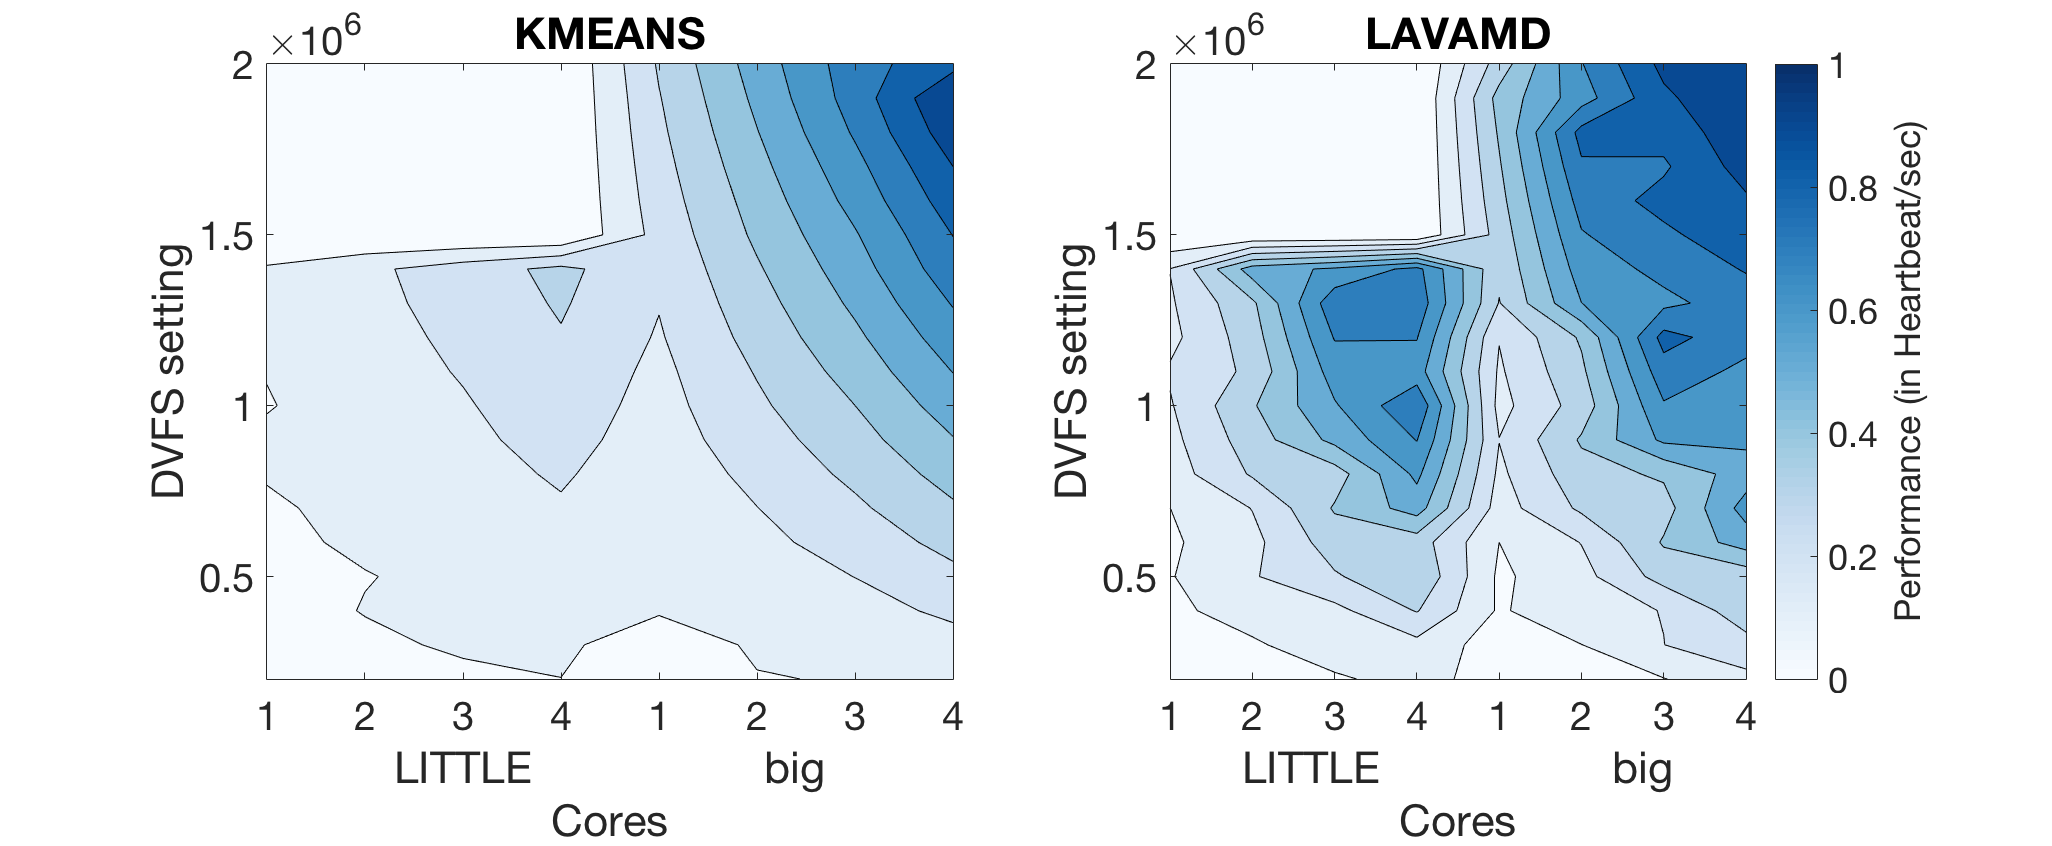
\includegraphics[width=\paperwidth,scale=0.5]{figures/performance-contour2.png}
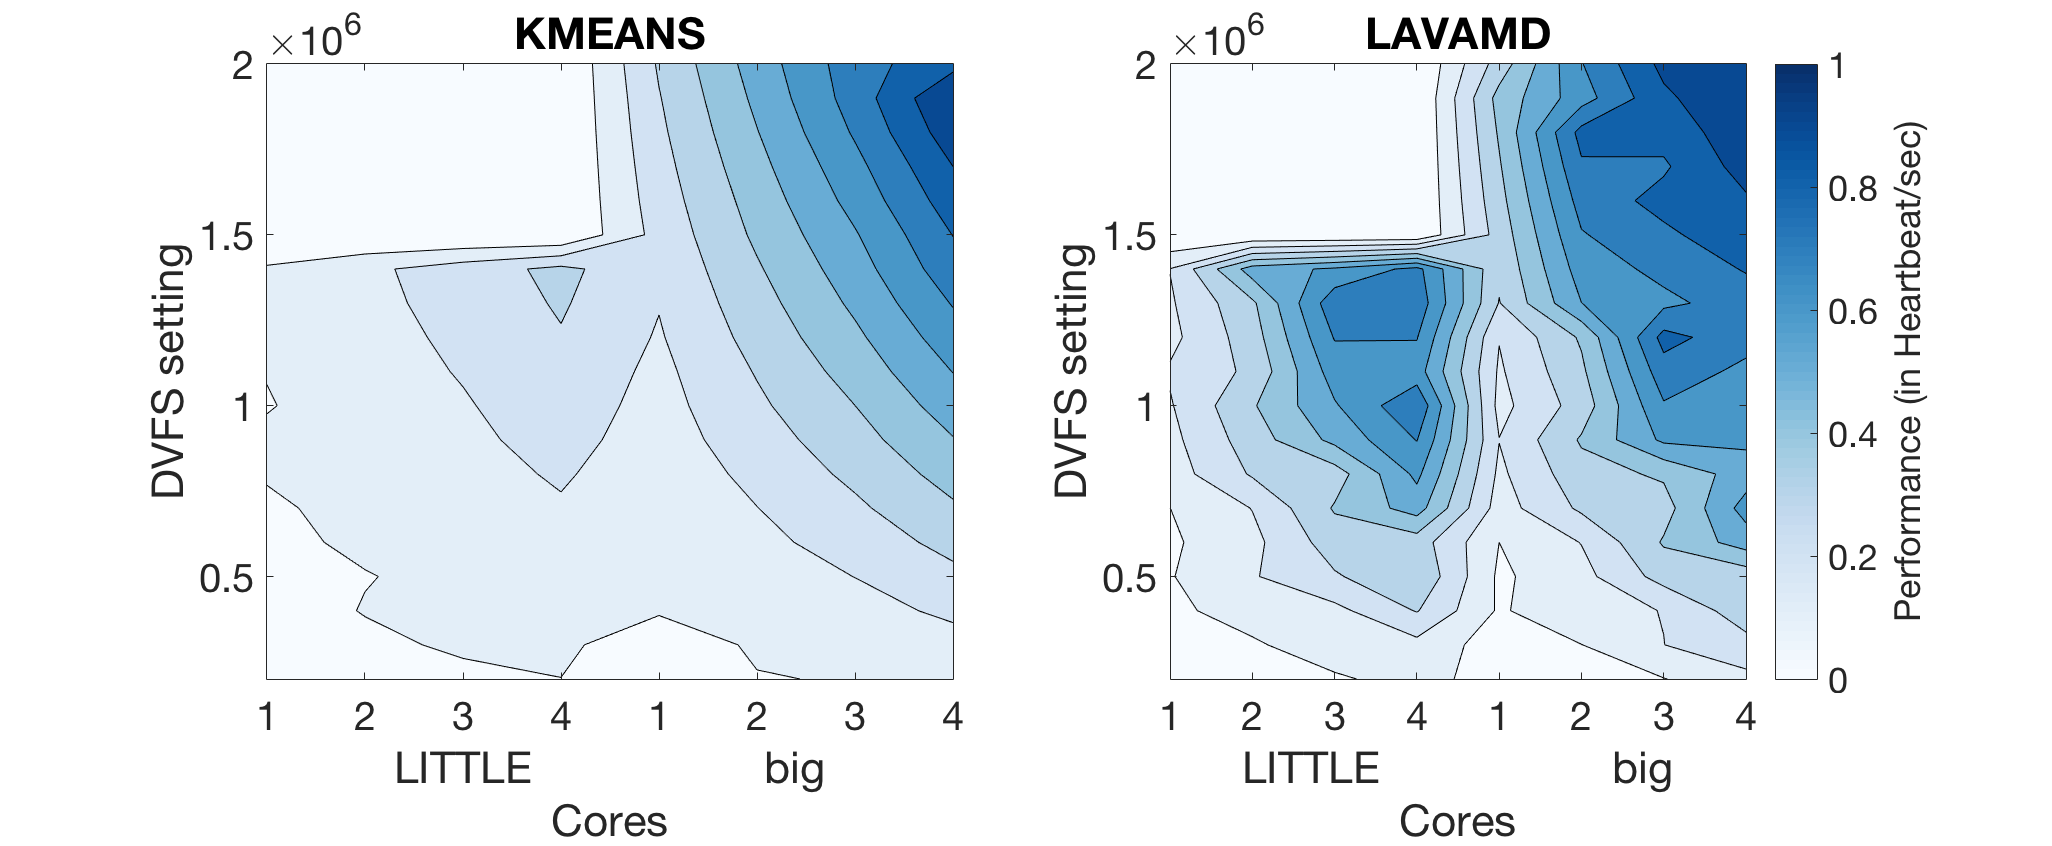
\includegraphics[width=\columnwidth]{figures/performance-contour2.png}
%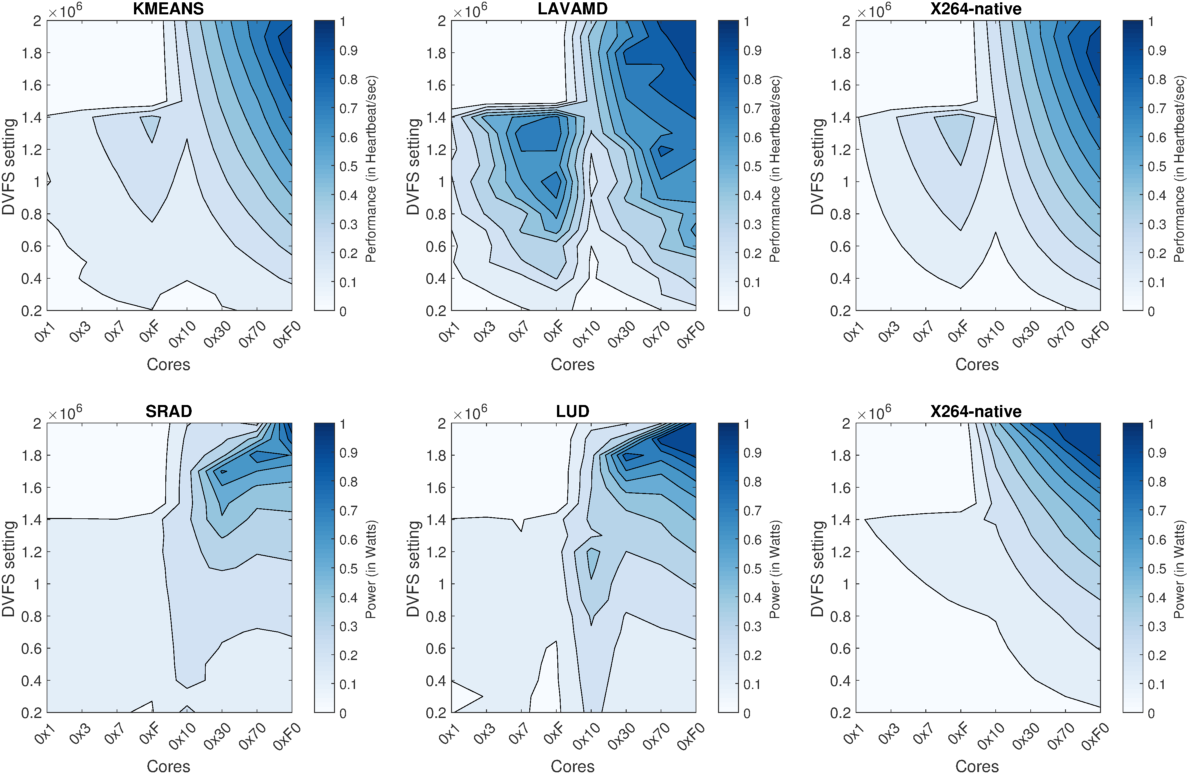
\includegraphics[scale=0.4]{figures/sample-contour3.png}
\caption{Contour plots showing performance as a function of core
  number, type, and speed.}
  \label{fig:contour}
\end{figure}
}

We consider prior \emph{learning} and \emph{control} approaches.  LEO,
a hierarchical Bayesian learner, estimates application performance as
a function of its resource usage \cite{LEO}. POET, a control system,
adjusts resource usage to meet application performance requirements
with minimal energy \cite{POET}.  This section develops intuition
about when one approach performs better than the other, motivating our
proposal to combine the two.

\subsection{\emph{Learning} Complexity}
Many machine learning approaches have been proposed to estimate
application performance in a variety of scenarios
\cite{reddiHPCA2013,LeeBrooks2006,CPR,ParallelismDial,Flicker,LeeBrooks,Koala}.
Machine learning is well suited to building models of complicated
systems like those shown in
\figsref{fig:lavamd_contour}{fig:kmeans_contour}.

To demonstrate how well learning manages complexity, we consider
meeting a performance requirement for \texttt{lavamd}, which has a
complicated configuration space.  We launch the application and use
either \emph{learning} or \emph{control} to meet a performance
requirement with minimal energy.  The \emph{learning} approach
estimates all configurations' performance and power and then uses the
lowest power configuration that delivers the required performance.
The \emph{control} approach has a generic model of performance/power
frontiers (similar to \texttt{kmeans}) and it constantly measures
performance and adjusts resource usage according to this generic
model.  \PUNT{While many controllers use linear models, POET uses a
  convex model and handles some non-linearities; however, it is
  sensitive to local maxima.}

\figref{fig:lavamd_timeline} shows the results of controlling 30
iterations of \texttt{lavamd} to meet the performance requirement.
The x-axis shows iteration number and the y-axis shows normalized
performance.  The learning approach achieves the goal, but the
controller oscillates wildly around it, sometimes not achieving the
goal and sometimes delivering performance that is too high (and wastes
energy). The oscillations occur because the controller adjusts
resources based on an incorrect (over-simplified) model of the
configuration space. Hence, the \emph{learner}'s ability to handle
complex models is crucial for reliable performance in this example.

%This result may be somewhat counter-intuitive.  The problem is that the controller cannot handle the complexity of \texttt{lavamd}.  One way to fix this problem would be to build a custom controller just for this application, but that controller would not be useful for other applications.  In contrast, the learner can find the local maxima in the configuration space, and as this application has no phase changes or other dynamics, the one configuration that the learner finds is suitable for the entire application.

\subsection{\emph{Controlling} Dynamics}
We now consider a dynamic environment.  We begin with \texttt{kmeans}
as the only application running on the system.  Halfway through its
execution, we launch a second app on a big core, dynamically altering
resource availability.

\figref{fig:kmeans_timeline} shows the results of this experiment.
The vertical dashed line represents when the second application
begins.  The figure clearly shows the benefits of a control system in
this dynamic scenario.  After a small dip in performance, the
controller returns it back to the desired level.  The learning system
however, does not have any inherent mechanism to measure the change or
adapt to the altered performance.  While we could theoretically
relearn the configuration space whenever the environment changes,
doing so is impractical.

Control systems are a light-weight mechanism for managing such
dynamics \cite{Hellerstein2004a}. Control systems are resilient to
scale change in the system performance or power.  Many dynamic changes
reduce all configurations' performance almost uniformly, changing the
magnitude of performance without altering the relative difference
between configurations.  For this reason, control systems have proven
especially useful in webservers with fluctuating request rates
\cite{Horvarth,LuEtAl-2006a,SunDaiPan-2008a} and multimedia
applications with dynamically varying inputs
\cite{TCST,Agilos,grace2}.

%%
\PUNT{
\begin{figure}
\centering
%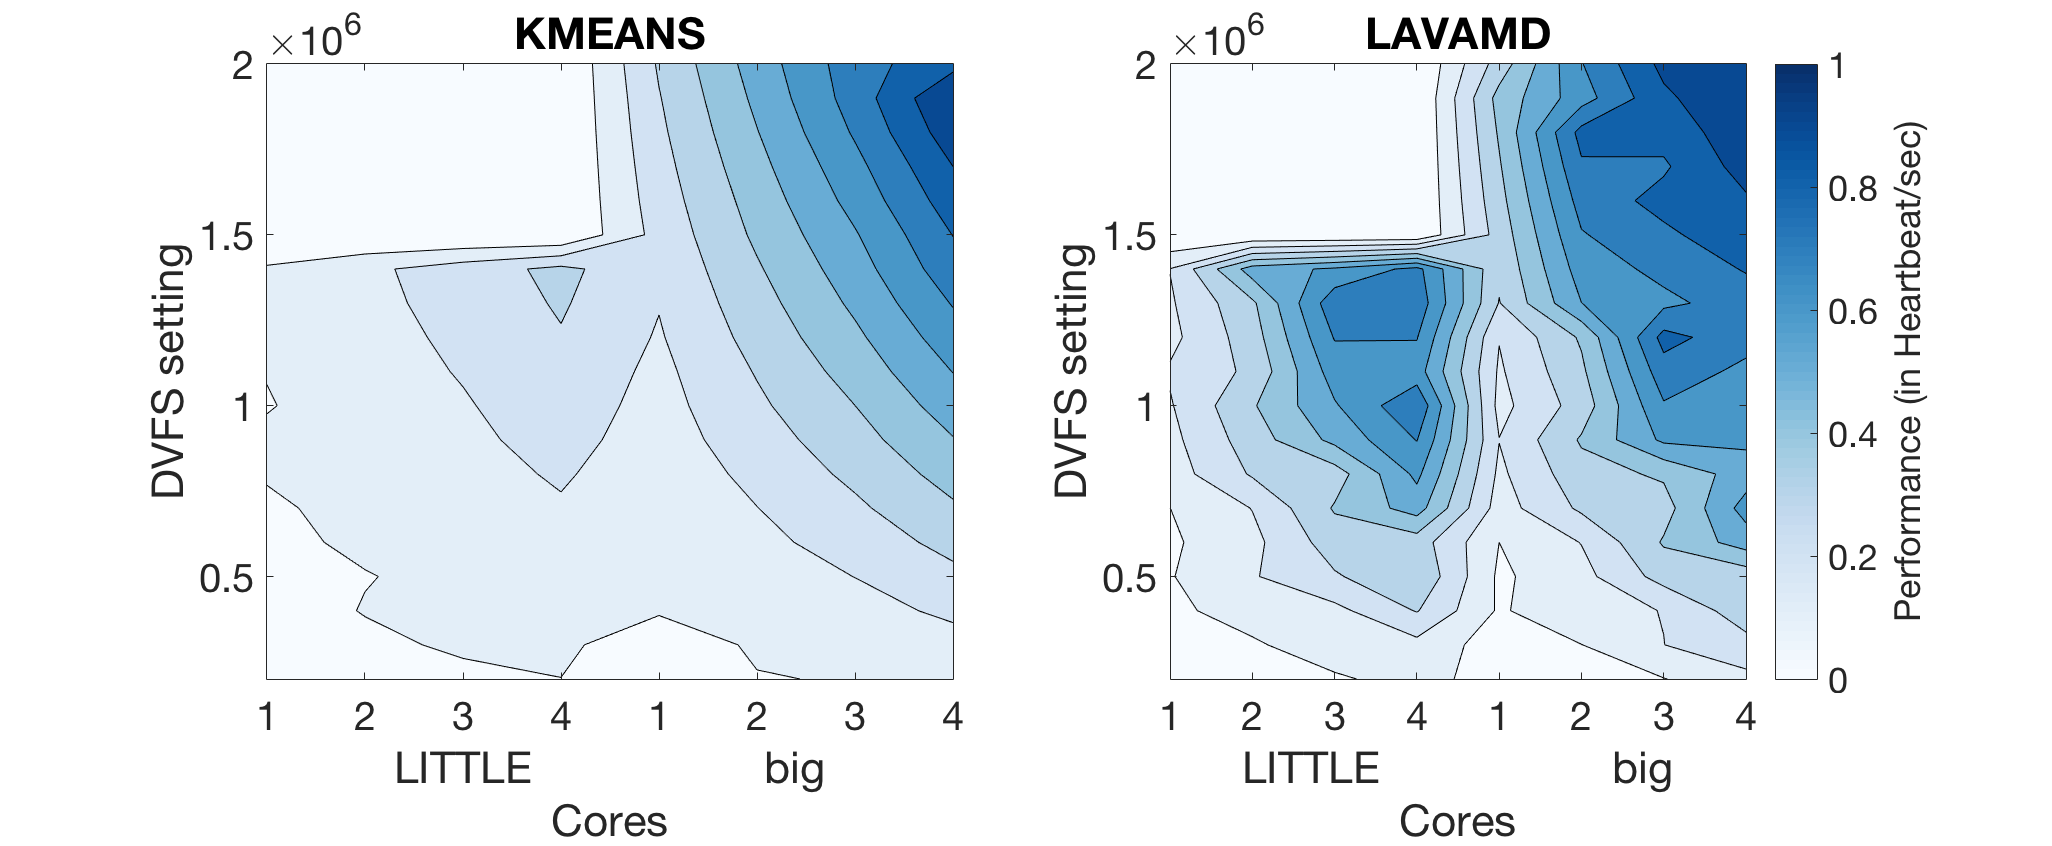
\includegraphics[width=\paperwidth,scale=0.5]{figures/performance-contour2.png}
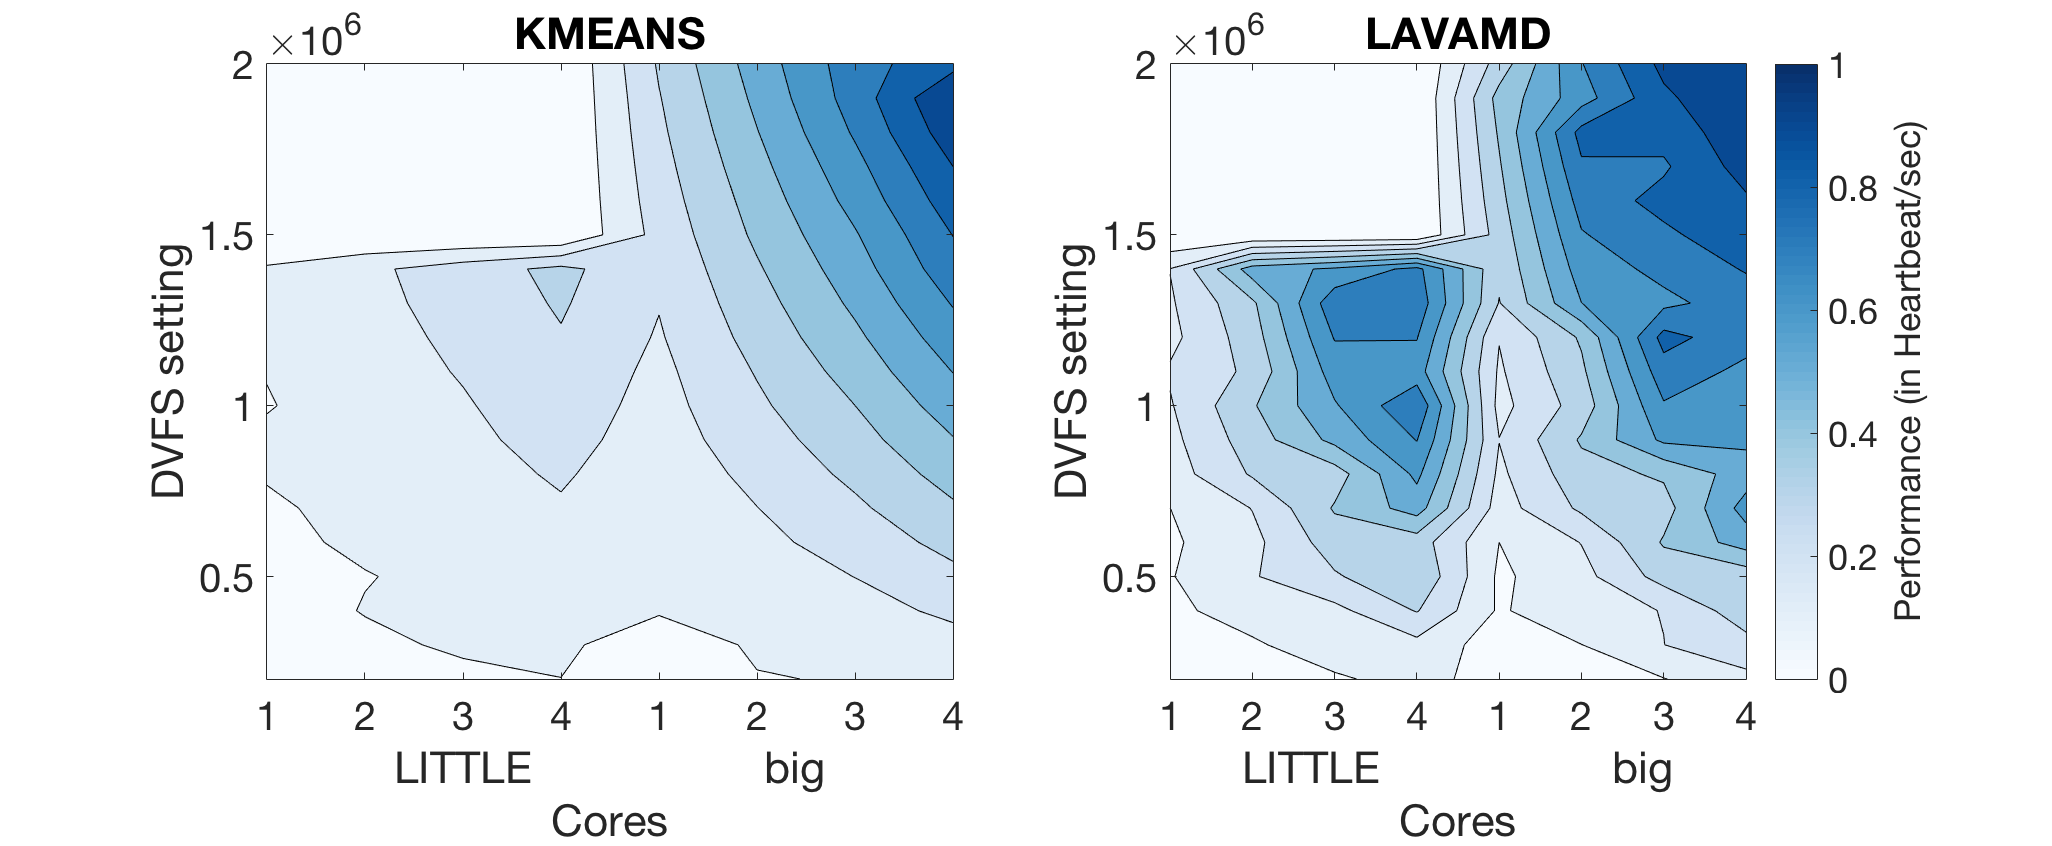
\includegraphics[width=\columnwidth]{figures/performance-contour2.png}
%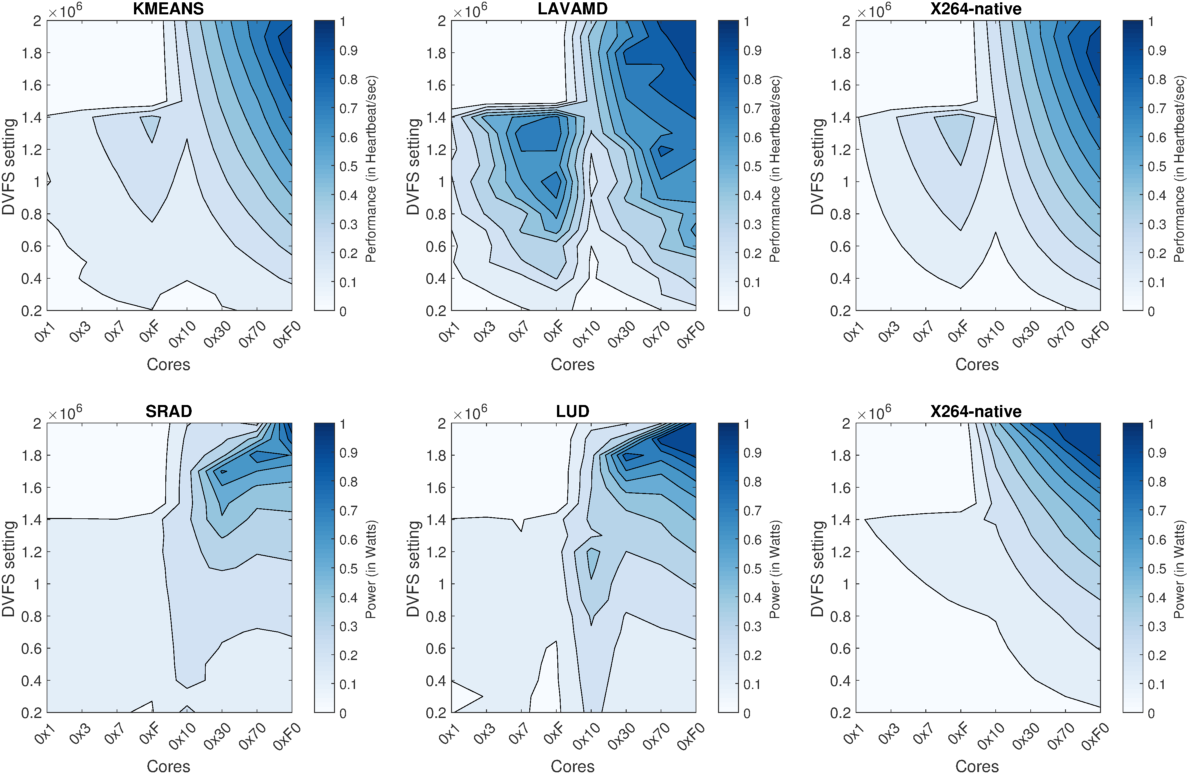
\includegraphics[scale=0.4]{figures/sample-contour3.png}
\caption{Contour plots showing performance as a function of core
  number, type, and speed.}
  \label{fig:contour}
\end{figure}

\begin{figure}[t]
  \begin{tikzpicture}
\begin{centering}

\definecolor{s1}{RGB}{228, 26, 28}
\definecolor{s2}{RGB}{55, 126, 184}
\definecolor{s3}{RGB}{77, 175, 74}
\definecolor{s4}{RGB}{152, 78, 163}
\definecolor{s5}{RGB}{255, 127, 0}

\begin{groupplot}[
    group style={
        group name=plots,
        group size=1 by 1,
        xlabels at=edge bottom,
        xticklabels at=edge bottom,
        vertical sep=5pt
    },
height=3.5cm,
width=0.95\columnwidth,
xmajorgrids,
ymajorgrids,
grid style={dashed},
xmin=0,
xmax=20,
yticklabel pos=left,
enlargelimits=false,
tick align = outside,
tick style={white},
xticklabel shift={-5pt},
yticklabel shift={-5pt},
ylabel shift={-2pt},
ylabel style={align=center},
unbounded coords=jump,
]

\nextgroupplot[ylabel={\footnotesize Performance \\ (Normalized)}, % Performance
%xtick={0,500,1000,1500,2000,2500,3000,3500,4000,4500},
ytick={0.0,0.5,1.0,1.5,2.0},
yticklabels={,0.5,1.0,1.5,2.0},
%xtick={0,30,60,120,160,200,240,280,320,480},
%xticklabels={,0,30,60,120,160,200,240,280,320,480},
yticklabel style={font=\footnotesize},
ymin=0,
ymax=1.5,
legend entries={,{$\mathsf{Learning}$},{$\mathsf{Control}$}},
legend style={draw=none,at={(0.5,1.4)},anchor=north,legend columns=4,line width=5pt},
]

\addplot[thick, dashed, black] coordinates {(10,0) (10,1.5)};
\addplot[thick, solid, color=s4] table[x index=0,y index=1,col sep=tab] {img/image_text/kmeans-example.txt};
\addplot[thick, solid, color=s5] table[x index=0,y index=2,col sep=tab] {img/image_text/kmeans-example.txt};
%\addplot[thick, dashed, black] coordinates {(130,0) (130, 2)};
\end{groupplot}
\end{centering}

\end{tikzpicture}

   \vskip -1em
  \caption{Performance Control for KMEANS}
  \label{fig:kmeans-example}
\end{figure}
}




